\documentclass[conference]{IEEEtran}
\usepackage{cite}
\usepackage{graphicx}
\usepackage{booktabs}
\usepackage{array}
\usepackage{url}
\graphicspath{{figures/}}
\usepackage{amsmath}
\usepackage{algorithm}
\usepackage{algpseudocode}
\newcolumntype{L}[1]{>{\raggedright\arraybackslash}p{#1}}

% vertical gaps before headings (tune the values to change the spacing)
\newcommand{\gapsection}{\vspace{1.2ex}}
\newcommand{\gapsubsection}{\vspace{0.5ex}}
\newcommand{\gapsubsub}{\vspace{0.4ex}}
% numbered heading on its own line (IEEEtran's \subsubsection runs into the text)
\newcommand{\subsubhead}[1]{\par\noindent\refstepcounter{subsubsection}%
{\normalfont\normalsize\itshape\arabic{subsubsection})\ #1}\par\nopagebreak}

\newcommand{\category}[1]{\par\vspace{0.6ex}\noindent\textbf{#1}\setcounter{subsubsection}{0}\par\nopagebreak}
\newcommand{\TR}{\par\noindent\textbf{Technical Requirements:}\par\nopagebreak}

\begin{document}
\setlength{\parskip}{1pt plus 1pt}

\title{SunSync: Proactive Daylight Control with\\Switchable Smart Film\\
\large Team SunSync}

\author{
\IEEEauthorblockN{\footnotesize 1\textsuperscript{st} Jiyeon Kim}
\IEEEauthorblockA{\footnotesize\textit{Dept. of Information Systems}\\
\footnotesize\textit{Hanyang University}\\
\footnotesize Seoul, South Korea\\
\footnotesize kjy8402@hanyang.ac.kr}
\and
\IEEEauthorblockN{\footnotesize 2\textsuperscript{nd} Daeun Lee}
\IEEEauthorblockA{\footnotesize\textit{Dept. of Information Systems}\\
\footnotesize\textit{Hanyang University}\\
\footnotesize Seoul, South Korea\\
\footnotesize daeun4862@hanyang.ac.kr}
\and
\IEEEauthorblockN{\footnotesize 3\textsuperscript{rd} Dain Lee}
\IEEEauthorblockA{\footnotesize\textit{Dept. of Information Systems}\\
\footnotesize\textit{Hanyang University}\\
\footnotesize Seoul, South Korea\\
\footnotesize ldi0308@hanyang.ac.kr}
\and
\IEEEauthorblockN{\footnotesize 4\textsuperscript{th} Heegyeong Chung}
\IEEEauthorblockA{\footnotesize\textit{Dept. of Information Systems}\\
\footnotesize\textit{Hanyang University}\\
\footnotesize Seoul, South Korea\\
\footnotesize hgchung04@gmail.com}
\and
\IEEEauthorblockN{\footnotesize 5\textsuperscript{th} Misong Ha}
\IEEEauthorblockA{\footnotesize\textit{Dept. of Information Systems}\\
\footnotesize\textit{Hanyang University}\\
\footnotesize Seoul, South Korea\\
\footnotesize msha9865@hanyang.ac.kr}
}

\maketitle

\begin{abstract}
Libraries with large windows face a recurring trade-off: direct sunlight fades and weakens paper-based collections, yet closing blinds takes daylight away from the whole reading room. UV-filtering films reduce part of the damage, and dynamic glass can tint ahead of changing conditions, but neither decides shading based on where light-sensitive objects are located in the room. We propose SunSync, a system that predicts where direct sunlight will fall inside a space and makes opaque only the cells of a switchable smart film through which the light would reach a protected target, before it arrives. Users register a space and measure its furniture with a mobile application that recognizes a QR marker displayed on the window film, and then set protected areas and protection grades on the web. A server calculates future sun positions, traces direct-sun paths from each protected surface through the window, and plans the state of each film cell. All other cells stay transparent, so the space keeps its daylight. Building on segmented PDLC and SPD films, the film is modeled as a grid of independently switchable cells and simulated in software. Although a library reading room is used as the main scenario, the same approach applies to museums, showrooms and homes.
\end{abstract}

\begin{IEEEkeywords}
proactive control, switchable smart film, daylighting, solar position, light damage, spatial measurement
\end{IEEEkeywords}

\begin{table}[!h]
\caption{Role Assignments}
\label{tab:roles}
\centering
\footnotesize
\setlength{\tabcolsep}{3pt}
\renewcommand{\arraystretch}{1.15}
\begin{tabular}{|L{0.2\columnwidth}|L{0.17\columnwidth}|L{0.48\columnwidth}|}
\hline
Roles & Name & Task description \\
\hline
Development Manager, Software Developer, Customer & Kim Jiyeon &
Project Management: Manages the schedule, the repository and issues.\newline
Requirements and Documentation: Writes the requirement, specification and design documents.\newline
Selective Shading (FR-02): Decides which film cells become opaque and when.\newline
Customer: Represents the target users and approves the deliverables. \\
\hline
Software Developer & Lee Daeun &
Spatial Measurement (FR-03): Designs the marker-based measurement of furniture positions and sizes.\newline
Data Integration: Converts the results into the space model and checks them against tape measurements. \\
\hline
User, UI/UX Designer & Lee Dain &
User Representative: Writes usage scenarios from a space manager's point of view and reviews usability.\newline
UI/UX Design and Front End: Designs and implements the mobile and web screens. \\
\hline
Software Developer & Chung Heegyeong &
Space Data (FR-06): Designs the space model shared by all modules and implements its validation and versioned storage API.\newline
Film Control (FR-05): Implements the virtual film, its interface and the application log. \\
\hline
Software Developer & Ha Misong &
Sunlight Prediction (FR-01): Implements sun position calculation and direct-sun path tracing.\newline
Prediction API: Provides the results to the applications and writes the verification scenarios. \\
\hline
\end{tabular}
\end{table}

\gapsection
\section{Introduction}
\gapsubsection
\subsection{Motivation}
This project is motivated by a conflict that many libraries face today: the need to protect their collections from light and the desire to offer readers a bright, daylit space.

\gapsubsub
\subsubhead{Light Damage Is Cumulative and Irreversible}
\noindent\hspace*{\parindent}Paper, inks, dyes and bindings deteriorate when exposed to light. The damage depends on the total exposure, which is the product of light intensity and time, and faded materials do not recover even when they are moved back into the dark \cite{nedcc,cci}. For this reason, conservation guidelines recommend that light-sensitive materials receive no more than about 50,000 lux hours per year and that collections be kept away from direct sunlight \cite{nedcc}. Since direct sunlight through a window can reach tens of thousands of lux, a shelf in the sun can use up this yearly budget within a short period.

\gapsubsub
\subsubhead{Libraries Want Daylight}
\noindent\hspace*{\parindent}At the same time, daylight and views are highly valued in library spaces. A study of library users found that readers appreciate windows that give visual relief from focused study, and concluded that the ideal library is ``a room with a view'' \cite{cam}. As a result, many libraries are designed with large glazed walls, and shelves and display cases are often placed near windows that receive direct sunlight for hours.

\gapsubsub
\subsubhead{Current Practice Solves Only Part of the Problem}
\noindent\hspace*{\parindent}Libraries currently rely on several measures against light damage. Clear UV-filtering films are widely installed; for example, Brown University's Rockefeller Library applied about 15,000 square feet of UV-blocking film to protect its rare books while keeping its transparent design \cite{solargard}. However, ultraviolet radiation accounts for only a part of the fading \cite{cci}, so visible light still reaches the collection. Tinted films reduce visible light but darken the window permanently, even when there is no direct sun. Blinds and shades are recommended during the most intense hours of sunlight \cite{nedcc}, yet they must cover the entire window to protect a single shelf, and they depend on staff operating them in time. Dynamic glass can tint parts of a facade or a pane in advance based on the sun's path and weather forecasts, but its control is designed around occupant glare, heat and energy \cite{view}. None of these approaches connects where sunlight will fall inside the room with what is located there.

\gapsubsub
\subsubhead{From Reactive to Proactive Control}
\noindent\hspace*{\parindent}Switchable films whose surface can be divided into independently controlled zones have appeared, such as LG Chem's switchable glazing film \cite{lgchem}, segmented PDLC and SPD glazing \cite{gauzyces} and films separated by thin laser-cut lines \cite{patent}. At the same time, the position of the sun can be calculated accurately for any future time \cite{pvlib,reda}, so the path of direct sunlight into a room can be predicted. What is still missing is software that decides which part of the window should be shaded, and when.

Used together with a UV-filtering film, SunSync predicts where direct sunlight will fall and makes opaque only the film cells through which that light would reach a protected target.

Although a library reading room is our main scenario, the same conflict exists wherever light-sensitive objects sit near windows, such as museums, cosmetics, perfume or wine showrooms, pop-up stores and homes. SunSync is therefore built on a general model of rooms, windows and protected targets that applies to these spaces without changing its core logic.

\gapsubsection
\subsection{Problem Statement}
Three problems remain in protecting collections from direct sunlight.

\gapsubsub
\subsubhead{Reactive and Manual Operation}
\noindent\hspace*{\parindent}In most reading rooms, blinds are lowered by staff when they notice sunlight on a shelf, which means the light has already reached the materials. Automated blinds that rely on light sensors also respond only after strong light is detected, and fixed schedules cannot follow the sun path, which shifts from day to day and season to season.

\gapsubsub
\subsubhead{All-or-Nothing Shading}
\noindent\hspace*{\parindent}Blinds and curtains treat a whole window as a single unit, and dynamic glass divides a pane into at most a few large zones. To keep sunlight off one bookshelf, the entire window or a large part of it has to be covered, and the reading seats next to it lose their daylight as well. Librarians must choose between protecting the collection and keeping the room bright, even when only a small part of the window causes the problem.

\gapsubsub
\subsubhead{No Awareness of What Needs Protection}
\noindent\hspace*{\parindent}Existing shading systems make decisions based on conditions outside or at the window, such as sun position, light level or glare on occupants. They do not know where valuable materials are placed in the room, how sensitive each one is, or which part of the window the harmful light passes through. As a result, they cannot shade selectively for the collection, and the decision of when and how much to shade is still left to the staff.

\gapsubsection
\subsection{Proposed Solution}
SunSync addresses these problems with three corresponding solutions.

\gapsubsub
\subsubhead{Predictive Sunlight Path Analysis}
\noindent\hspace*{\parindent}Instead of waiting for sunlight to appear, SunSync calculates the position of the sun for upcoming time steps and traces the path of direct sunlight from each protected surface back through the window. This tells the system in advance whether, when, and through which point of the window sunlight will reach each target, so that shading can be applied before exposure begins.

\gapsubsub
\subsubhead{Cell-Level Selective Shading}
\noindent\hspace*{\parindent}SunSync maps the predicted light paths onto the cells of a switchable film and makes opaque only the cells that would let sunlight reach a protected target. All other cells stay transparent, so the rest of the room keeps its daylight.

\gapsubsub
\subsubhead{Target-Aware Protection Settings}
\noindent\hspace*{\parindent}The librarian measures the room with the mobile application, marks the areas to protect on the web, and gives each area a protection grade, from strict blocking of direct sunlight to daylight priority. SunSync uses these settings to decide which cells to shade and when.

These solutions rely on switchable films that are commercially available. Polymer-dispersed liquid crystal (PDLC) film scatters light when unpowered and turns clear within about 10 to 150 ms when a voltage is applied \cite{gauzypdlc}. Suspended particle device (SPD) film absorbs light instead and can block up to 99\%, but it switches more slowly (up to about 3 seconds) and allows gradual tint control \cite{gauzypdlc,solarscreen}. Both are sold with zones, such as PDLC windows with segment control and SPD windows with five separately controlled segments \cite{gauzyces}, but since each segment needs its own electrical connection, current products remain at a few segments or strip patterns. SunSync assumes that this segmentation is extended to a grid of small cells, so that the shaded area for each target shrinks to the cells its sunlight passes through; in this project, a 1 m $\times$ 1 m window is divided into 10 $\times$ 10 cells of 10 cm. The main scenario uses PDLC, whose opaque state spreads the direct beam into diffuse light so that no concentrated sun patch reaches the target; SPD can be used where the light itself must be reduced. Because such cell grids are not yet sold, the film is simulated in software in this project, and sunlight intensity is estimated under clear-sky conditions when weather forecasts are not used.

\gapsubsection
\subsection{Research on Related Software}
SunSync builds on several existing products and technologies that control or analyze daylight:

\gapsubsub
\subsubhead{Switchable Smart Films}
\noindent\hspace*{\parindent}LG Chem has developed a switchable glazing film for vehicle sunroofs that stays opaque without power and becomes transparent when a voltage is applied, and the glass can be divided into zones that are set transparent or opaque separately \cite{lgchem}. Segmented films, in which thin laser-cut lines divide one film into independently switchable areas, are described in patents and offered commercially \cite{patent,gauzyces}. These films provide the zone-level hardware that SunSync assumes, but in current products the user chooses which zone to switch.

\gapsubsub
\subsubhead{Dynamic Glass with Zoned Tinting}
\noindent\hspace*{\parindent}Electrochromic dynamic glass changes its tint automatically to manage daylight, glare and heat. View Intelligence combines the sun's path, rooftop sensors and weather forecasts to tint windows in advance, and windows can be grouped into zones or facades \cite{view}. SageGlass offers up to three tint zones, or a vertical tint gradient, within a single pane \cite{sageglass}. These systems control parts of a facade or a pane and act ahead of changing conditions, but their control is designed mainly around occupant comfort and energy and does not consider the location and sensitivity of objects inside the room.

\gapsubsub
\subsubhead{Automated Shading Systems}
\noindent\hspace*{\parindent}Automated shade systems such as MechoSystems SolarTrac adjust motorized shades according to the sun's position, the direction of solar rays and the sky conditions measured by radiometers, aiming to maximize daylight while preserving views \cite{mecho}. They move a whole shade along the window, so a single shade position applies to the entire area behind it.

\gapsubsub
\subsubhead{Smart Home Platforms and AI Home Hubs}
\noindent\hspace*{\parindent}Google Home and Apple Home let users close smart blinds with routines triggered by time, sunrise or sunset, and LG introduced ThinQ ON as a Matter-certified hub that connects devices from other manufacturers, learns usage patterns and runs automation routines \cite{thinq}. These platforms are moving toward proactive control of the whole home, but they rely on schedules, device states and usage patterns rather than on where sunlight falls in a room. SunSync can complement them by supplying sunlight prediction and protection logic, and its decisions could be delivered to such hubs through Matter, which already defines window coverings as a device type.

\gapsubsub
\subsubhead{Solar Position and Daylight Calculation Tools}
\noindent\hspace*{\parindent}pvlib is an open-source Python library that implements the NREL Solar Position Algorithm and related solar models \cite{pvlib,reda}, and Radiance, developed at Lawrence Berkeley National Laboratory, is widely used to simulate daylight inside buildings \cite{radiance}. Such tools are mainly used for analysis and design. SunSync uses pvlib for its sun position calculations.

\gapsection
\section{Requirements}
\gapsubsection
\subsection{Mobile Application Requirements (MAR)}
\subsubhead{MAR1. Sign In}
\noindent\hspace*{\parindent}Users sign in with an account that is shared by the mobile and web applications, so that a space registered on one is available on the other. % TODO: Google sign in is the target; the current prototype uses a demo account

\subsubhead{MAR2. Space Registration}
\begin{itemize}
\item \textit{MAR2.1 Space Information:} The user enters the building name, floor and space name. The location (latitude, longitude, time zone) is filled in from the position of the device and can be edited, and the user confirms the north direction.
\item \textit{MAR2.2 Space Size:} The user enters the width, depth and height of the space in metres.
\item \textit{MAR2.3 Zones:} A large space can be divided into several zones. Each zone is registered and measured separately, and zones can be added and deleted.
\item \textit{MAR2.4 Window:} The user enters the size of the window, the wall that it is on, its distance from the end of the wall and the height of its lower edge. The size and position of the marker on the film are entered with a preview of the film cells.
\end{itemize}

\subsubhead{MAR3. Marker-Based Measurement}
\begin{itemize}
\item \textit{MAR3.1 Measurement Request:} A measurement starts from a request that is linked to the account. The request is made on the web or in the application, and the application lists the waiting requests. A link or a QR code can open a request directly.
\item \textit{MAR3.2 Corner Capture:} The user enters the name and type of a piece of furniture and photographs the marker from each of its four corners in a guided order. The application checks blur and brightness on the device and asks for a retake with the reason. Several pieces of furniture can be measured one after another, and the values can also be entered directly. No video is recorded.
\item \textit{MAR3.3 Transfer:} The measurement data are sent to the server, and the progress of the floor plan generation is displayed.
\end{itemize}

\subsubhead{MAR4. Floor Plan Check}
\noindent\hspace*{\parindent}The application shows the generated floor plan with the position of the window and the furniture. The user can select a piece of furniture, change its type, size, height and position, drag it on the plan, add or delete furniture, and save the result. A link opens the same space on the web to continue with the protected areas.

\subsubhead{MAR5. Space Status}
\begin{itemize}
\item \textit{MAR5.1 Sunlight by Time:} The floor plan shows the predicted exposure of the protected areas, and a time slider lets the user follow it during the day.
\item \textit{MAR5.2 Protected Areas:} The protected areas and their grades are displayed, and they can be edited in the mobile application as well as on the web.
\item \textit{MAR5.3 Film State:} The window is displayed as a grid of film cells, and the cells that are opaque at the selected time are highlighted.
\item \textit{MAR5.4 Shading Hours:} The user can turn shading on or off and set its start and end time in steps of 10 minutes. The film is shaded only within these hours. % NOTE: the setting exists in the UI; check whether the server applies it
\end{itemize}

\gapsubsection
\subsection{Web Application Requirements (WAR)}
\subsubhead{WAR1. Account and My Spaces}
\noindent\hspace*{\parindent}Users sign in with the same account as in the mobile application. The web application lists the registered spaces by building, and the user can add, open or delete a space.

\subsubhead{WAR2. Space Registration}
\noindent\hspace*{\parindent}The user enters the same space information, size, zones and window as in MAR2. The web application creates a measurement request for the mobile application (MAR3.1); it has no camera input of its own.

\subsubhead{WAR3. Floor Plan and Protected Area Editing}
\begin{itemize}
\item \textit{WAR3.1 Furniture:} The user selects furniture on the floor plan and corrects its type, width, depth, height and position. Furniture can be added by marker measurement or by direct input, and it can be deleted.
\item \textit{WAR3.2 Protected Areas:} The user creates a protected area by selecting a face of a piece of furniture or by drawing an area on the floor plan, and sets its start and end height and its protection grade (A to D). An area can be moved and resized by dragging or by entering numbers.
\item \textit{WAR3.3 3D View:} The measured space can be viewed in 3D, with a default shape for each furniture type, and furniture can be moved by dragging. % TODO: planned, not yet implemented
\item \textit{WAR3.4 Saving:} Changes are saved to the server. The application warns before the user leaves unsaved changes and shows the newest content if the server refuses a version.
\end{itemize}

\subsubhead{WAR4. Space Status}
\begin{itemize}
\item \textit{WAR4.1 Overview:} For each zone, the web application shows the floor plan with furniture, protected areas and the predicted exposure. It shows whether the intensity comes from a forecast or from the clear-sky value.
\item \textit{WAR4.2 Shading Schedule:} It shows the time at which light toward each protected area is expected to be blocked, and the user can request a recalculation.
\item \textit{WAR4.3 Film State:} The window is displayed as a grid of film cells, and the cells that are opaque at the selected time are highlighted.
\item \textit{WAR4.4 Shading Hours:} The user sets the shading hours as in MAR5.4.
\end{itemize}

\gapsubsection
\subsection{Functional Requirements (FR)}
\subsubhead{FR-01. Future Sunlight Path Prediction}
\noindent\hspace*{\parindent}The system must predict, for a future time window, whether direct sunlight reaches each protected area, when it first arrives, through which point of the window, and how strong it is.
\begin{itemize}
\item \textit{FR-01.1 Solar Position:} Calculate the elevation and azimuth of the sun for each time step from the location of the space and a time zone-aware start time.
\item \textit{FR-01.2 Direct-Sun Path Tracing:} Divide each protected area into tiles of 5 cm $\times$ 5 cm and, from the centre of each tile, trace a ray toward the sun and check whether it leaves the room through a window without being blocked by a wall or furniture. For a valid path, return the window and the crossing point in ENU coordinates.
\item \textit{FR-01.3 Exposure Timeline:} Return, for each time step, whether each tile is exposed and why, and the first predicted exposure time of each protected area.
\item \textit{FR-01.4 Sunlight Intensity:} For each time step, select the direct normal irradiance from the Scene weather record, then from a stored Open-Meteo forecast, then from the pvlib clear-sky value, otherwise unknown, and convert it to the direct irradiance on each tile.
\end{itemize}

\subsubhead{FR-02. Selective Shading Decision}
\noindent\hspace*{\parindent}The system must make opaque only the film cells through which direct sunlight would reach a protected area, and keep all other cells transparent.
\begin{itemize}
\item \textit{FR-02.1 Cell Mapping:} Expand each window crossing point by 2.5 cm in each direction in window coordinates and return every film cell that the expanded area overlaps.
\item \textit{FR-02.2 Grade-Based Decision:} Apply the protection grade of each area (FR-06.6). Grade A shades every cell that a direct-sun path reaches, whatever the intensity. For grades B and C, the largest tile irradiance of an area in a cell is compared with the limit of the grade, and the result is opaque, infeasible when the film cannot meet the limit, or unknown when the intensity is unknown. When a cell affects several areas, the most severe state applies.
\item \textit{FR-02.3 Advance Shading:} Switch a cell before the predicted arrival time, allowing for the switching time of the film, processing delay and a safety margin.
\item \textit{FR-02.4 Shading Schedule:} Provide the planned cell states over time, with the reasons, to the mobile and web applications as a shading plan through \texttt{POST /api/scenes/\allowbreak\{scene\_id\}/\allowbreak shading-plans}.
\end{itemize}

\subsubhead{FR-03. Marker-Based Spatial Measurement}
\noindent\hspace*{\parindent}The system must estimate the positions and sizes of furniture from photos of a marker of known size and position, taken at measuring points on the furniture.
\begin{itemize}
\item \textit{FR-03.1 Marker Detection:} Detect the ArUco marker in each photo and check the image quality, such as blur or partial occlusion. Reject photos in which the marker is not fully visible.
\item \textit{FR-03.2 Camera Position Estimation:} For each photo, calculate the 3D position and orientation of the camera from the known marker size and its corners. The camera position is the coordinate of the measuring point.
\item \textit{FR-03.3 Furniture Output:} Fit the shape of the furniture to the measuring points, which gives its width, depth, position and rotation, determine its height, convert the result to ENU coordinates, and register it in the Scene for the user to review.
\end{itemize}

\subsubhead{FR-05. Film Control Interface}
\noindent\hspace*{\parindent}The system must send its decisions to the film through a device interface. In this project the film is simulated in software as a grid of independently switchable cells.
\begin{itemize}
\item \textit{FR-05.1 Cell Commands:} Apply the planned state of each cell at the scheduled time, record every change, and return the state of the film at any requested time.
\item \textit{FR-05.2 Marker Display:} During measurement, display the marker board of FR-03 on a fixed block of film cells and restore the previous cell states afterward.
\item \textit{FR-05.3 Replaceable Device:} Keep the interface independent of the film hardware and film type, such as PDLC or SPD, so that the simulated film can later be replaced by a real controller.
\end{itemize}

\subsubhead{FR-06. Space Information Management}
\noindent\hspace*{\parindent}The system must store each space as a versioned model in metres, in a coordinate frame where x points east, y points north and z points up, with the floor at $z = 0$.
\begin{itemize}
\item \textit{FR-06.1 Space Model:} Store the location, room size, zones, windows with their film cell layout, furniture as boxes with a furniture type, an optional floor level, and protected areas as rectangles of four vertices with their grades; sample points are generated by FR-01 and are not stored.
\item \textit{FR-06.2 Window Specification:} Store the window size and position entered by the user, together with the block of film cells on which the marker is displayed (start row and column, number of rows and columns); the physical size of the marker follows from the cell size.
\item \textit{FR-06.3 Measurement Records:} Record whether each value was entered manually or measured with the marker, with the time of the measurement.
\item \textit{FR-06.4 Validation and Versioning:} Reject invalid geometry with an explanation, increase the version on every update, and prevent two users from overwriting each other's changes.
\item \textit{FR-06.5 Synchronization:} Provide the same space data to the mobile and web applications.
\item \textit{FR-06.6 Protection Grades:} Each protected area has one of four grades. Grade A requires every geometric direct-sun path to the surface to pass through an opaque cell, even when the predicted intensity is low or unknown. Grades B and C limit the direct sunlight intensity on the surface to a low and a higher configurable value (30 and 70 W/m$^2$ in the demonstration). Grade D gives priority to daylight and makes no shading request.
\end{itemize}

\gapsubsection
\subsection{Non-Functional Requirements (NFR)}
\subsubhead{NFR1. Accuracy and Stability}
\begin{itemize}
\item \textit{NFR1.1 Reference Agreement:} Predicted first exposure times must agree with hand-calculated reference cases within one time step, and all inputs must carry units, time zones and reference directions.
\end{itemize}

\subsubhead{NFR2. Performance and Usability}
\begin{itemize}
\item \textit{NFR2.1 Calculation Time:} A two-hour plan for one zone must be calculated within 5 seconds.
\item \textit{NFR2.2 Responsive and Guided Use:} The applications must work on phone and PC screens, and each step must explain what to do next.
\end{itemize}

\subsubhead{NFR3. Data Consistency}
\begin{itemize}
\item \textit{NFR3.1 Shared and Reproducible Data:} A space saved on one device must appear the same on the other, and the same inputs must produce the same result.
\end{itemize}

\gapsection
\section{Development Environment}
\gapsubsection
\subsection{Choice of Software Development Platform}
\category{Platform}
\subsubhead{Web (Progressive Web Application)}
\noindent\hspace*{\parindent}SunSync is built as a web-based system: a Python server and a responsive progressive web application (PWA) that runs in the browser of phones and PCs from one code base. A PWA needs no app-store installation and can use the phone camera, which the marker photos require. Native iOS and Android applications would need two code bases and developer accounts, and the schedule and budget of this project do not allow that. The film is a virtual device, so no hardware platform is involved.

\category{Programming Languages}
\subsubhead{Python \cite{python}}
\noindent\hspace*{\parindent}Python is a high-level programming language with a large ecosystem of scientific and geometry libraries. The solar position (pvlib), planar geometry (shapely) and marker detection (OpenCV) libraries of SunSync are Python libraries, so the server, the prediction engine, the shading decision, the film control and the measurement module are written in Python 3.11 or later and run in one environment.

\subsubhead{TypeScript \cite{typescript}}
\noindent\hspace*{\parindent}TypeScript is a typed superset of JavaScript that checks types at compile time. SunSync uses it for the web and mobile client, so that the data exchanged with the server (Scene, prediction, shading plan) is checked against its type before the code runs.

\category{Development Tools}
\subsubhead{GitHub \cite{github}}
\noindent\hspace*{\parindent}GitHub hosts the Git repository of the project. SunSync uses it for version control, pull request review, issues in the user story format, the project board and the milestones of the sprints. Documents, API descriptions, data contracts and the decisions of the team are kept in the repository next to the code.

\subsubhead{GitHub Actions \cite{githubactions}}
\noindent\hspace*{\parindent}GitHub Actions runs automated workflows on each push and pull request. The workflow of SunSync checks the server with ruff, mypy and pytest on Python 3.11 and 3.12, tests the measurement module, and checks the client with a lint, tests and a build.

\subsubhead{pytest, ruff, mypy and oxlint \cite{pytest,ruff,mypy,oxlint}}
\noindent\hspace*{\parindent}pytest runs the automated tests of the Python code, ruff checks and formats it, and mypy checks its types. oxlint checks the TypeScript code of the client. The workflow of GitHub Actions runs these checks on every change.

\subsubhead{Overleaf \cite{overleaf}}
\noindent\hspace*{\parindent}Overleaf is an online LaTeX editor. The requirement and specification documents are written in the IEEE conference template on Overleaf, and their LaTeX sources are stored in the repository.

\subsubhead{Google Docs \cite{gdocs}}
\noindent\hspace*{\parindent}Google Docs is an online document editor. The meeting notes of the team are kept in a shared Google document, while all other documents are kept in the repository.

\category{Frameworks}
\subsubhead{FastAPI \cite{fastapi}}
\noindent\hspace*{\parindent}FastAPI is a Python web framework that builds typed HTTP routes and generates API documentation automatically. SunSync uses it for all server routes, together with Pydantic models that validate every request and response.

\subsubhead{React and Vite \cite{react,vite}}
\noindent\hspace*{\parindent}React is a JavaScript library for building user interfaces from components, and Vite is a build tool with fast development builds. They are used to build the responsive web application that runs as a progressive web application (PWA) on phones and PCs from one code base, without an app-store installation.

\category{Cost Estimation}
\noindent\hspace*{\parindent}SunSync uses open-source software and the free tiers of its services. The film is simulated in software, so no hardware is purchased. The only paid items are the subscriptions of development assistance tools that some members hold. Table~\ref{tab:cost} shows the estimated cost.

\begin{table}[!t]
\caption{Development and Deployment Cost Estimation}
\label{tab:cost}
\centering
\footnotesize
\setlength{\tabcolsep}{3pt}
\renewcommand{\arraystretch}{1.15}
\begin{tabular}{|L{0.24\columnwidth}|L{0.34\columnwidth}|L{0.22\columnwidth}|}
\hline
Category & Item & Cost (KRW) \\
\hline
Cloud infrastructure & None (local server) & 0 \\
\hline
Development tools & GitHub, GitHub Actions, Overleaf, Google Docs, test and lint tools & 0 \\
\hline
Software & Python, TypeScript, FastAPI, React, Vite, pvlib, OpenCV, shapely, SQLite & 0 \\
\hline
Data & Open-Meteo forecast & 0 \\
\hline
Hardware & PCs and smartphones of the members & 0 \\
\hline
Development assistance & Subscriptions of development assistance tools & 29,000 per month each \\
\hline
Total & & 29,000 per month per subscription \\
\hline
\end{tabular}
\end{table}

\noindent\textbf{Cost Breakdown Notes:}
\begin{itemize}
\item Software: all libraries are open source and have no licensing cost.
\item Development tools: the free tiers are used; Overleaf is used on the free plan by one editor.
\item Data: Open-Meteo is free for non-commercial use \cite{openmeteo}.
\item Hardware: the PCs and phones that the members already own are used, and no film hardware is purchased.
\item Development assistance: some members pay for subscriptions of development assistance tools themselves (29,000 KRW per month for each current subscription), and one more subscription is planned. % TODO: confirm the number of subscriptions and the price of the planned one
\item Cloud: no commercial cloud platform is used at present; a demonstration is run on a local server.
\end{itemize}

\category{Development Environment}
\noindent\hspace*{\parindent}Table~\ref{tab:env} lists the versions of the development environment.

\begin{table}[!t]
\caption{Development Environment}
\label{tab:env}
\centering
\footnotesize
\setlength{\tabcolsep}{3pt}
\renewcommand{\arraystretch}{1.15}
\begin{tabular}{|L{0.3\columnwidth}|L{0.57\columnwidth}|}
\hline
Item & Value \\
\hline
Server runtime & Python 3.11 and 3.12 (both run in CI) \\
\hline
Client runtime & Node.js 24, React 19, Vite 8, TypeScript 6 \\
\hline
Database & SQLite (WAL mode) \\
\hline
CI environment & GitHub Actions, ubuntu-latest \\
\hline
Operating systems & macOS and Windows % TODO: versions
\\
\hline
Computers (macOS) & MacBook Pro (M2 Pro, 32 GB), Mac Studio (M2 Max, 32 GB), MacBook Air (M2, 8 GB), MacBook Air (M4, 16 GB) \\
\hline
Computers (Windows) & Laptop (Intel Core i7-1360P, 16 GB RAM, NVIDIA RTX 3050 4 GB); desktop (Intel Core i7-14700K, 64 GB RAM, NVIDIA RTX 4080 SUPER 16 GB) \\
\hline
\end{tabular}
\end{table}

\gapsubsection
\subsection{Software in Use}
\category{Libraries and Services}
\subsubhead{pvlib \cite{pvlib,reda}}
\noindent\hspace*{\parindent}pvlib is an open-source Python library that implements the NREL Solar Position Algorithm and clear-sky irradiance models. In SunSync, it calculates the elevation and azimuth of the sun for every time step, and it provides the clear-sky direct normal irradiance (DNI) that is used when no forecast is available.

\subsubhead{Open-Meteo \cite{openmeteo}}
\noindent\hspace*{\parindent}Open-Meteo is a weather forecast service with an HTTP interface. SunSync requests the hourly DNI and cloud cover for the location of each stored space. Each DNI value is the mean of the preceding hour. A separate worker stores the responses in the database, so that a prediction request never calls the service.

\subsubhead{OpenCV and ArUco markers \cite{opencv,garrido}}
\noindent\hspace*{\parindent}OpenCV is a computer vision library. Its ArUco module detects square markers with a binary pattern, and its perspective-n-point solver (solvePnP) computes the camera position and orientation from the corners of a marker of known size. SunSync uses the $4\times4$ dictionary to measure the furniture, and it also draws the marker on the cells of the virtual film.

\subsubhead{shapely \cite{shapely}}
\noindent\hspace*{\parindent}shapely is a Python library for planar geometry. SunSync uses it for polygon operations, such as the footprint of the room and the fitting of a rectangle to measured points.

\subsubhead{Pydantic, SQLModel and SQLite \cite{pydantic,sqlmodel,sqlite}}
\noindent\hspace*{\parindent}Pydantic describes the data models in code and validates them, SQLModel maps them to tables, and SQLite is a file-based database that needs no installation. In SunSync, the Scene, the shading plan and the film commands are Pydantic models, and the Scenes, forecast records, film states and application logs are stored in SQLite.

\subsubhead{Three.js \cite{threejs}}
\noindent\hspace*{\parindent}Three.js is a JavaScript library for 3D graphics in the browser. It is planned for the 3D view of the measured space in the web application.

\gapsection
\section{Specifications}
This section defines the functional specifications of the SunSync system, organized by feature categories. Each specification describes the technical requirements and the implementation details necessary for system operation. All coordinates are in metres in a right-handed ENU frame (x east, y north, z up) with the floor at $z=0$. The film of a window is a grid of cells whose origin $(0,0)$ is the top-left cell seen from inside; the default grid is $10\times10$ cells of 10 cm.

\gapsubsection
\subsection{Space Registration and Management Features}
\subsubhead{Account and Sign In (planned)}
\noindent\hspace*{\parindent}Users sign in with one account in the mobile and the web application, so that a space is available on both. The screens for sign in exist as a demonstration; the server does not yet check an account.

\TR
\begin{itemize}
\item Sign in with a Google account by OAuth 2.0; the client sends the ID token to the server, which verifies it and opens a session
\item The account owns its spaces; a request for a space of another account is refused
\item Until this is implemented, the demonstration screens keep a local demo account, and the data on the development server are not separated by user
\end{itemize}

\subsubhead{My Spaces}
\noindent\hspace*{\parindent}The list of spaces is the starting point of the registration, the measurement and the status screens. The web application shows the spaces as cards, and the mobile application shows them in the space tab.

\TR
\begin{itemize}
\item The list is grouped by building and can be searched by name; each card shows the plan, the state (protected areas set or not) and whether the space is saved on the server
\item Actions: open, register a new space, delete a space
\item The list reads \texttt{GET /api/ui/spaces}; a space without the screen data of the application is listed as unavailable and is not converted or overwritten
\item Waiting measurement requests are shown with the space and refreshed every 3 seconds
\end{itemize}

\subsubhead{Space Registration}
\noindent\hspace*{\parindent}The registration screen collects the information that all other functions need: the names of the building, floor, space and zone, the size of the room, the window and the position of the marker. The location is filled in from the device and can be corrected. The location and the north direction are never filled in with an assumed value.

\TR
\begin{itemize}
\item Input: building, floor (integer from $-100$ to 1000), space and zone names; room width, depth and height (m); latitude, longitude and time zone; confirmation of the north direction
\item Window: width, height, wall, distance from the end of the wall, height of the lower edge; film grid (default $10\times10$ cells of 10 cm)
\item Marker: size and position on the film, shown as a preview of the film cells
\item A space is saved with \texttt{POST /api/ui/spaces}; the screen shows ``saved'' only after the server confirms, and keeps the entries if the connection fails or the input is invalid
\end{itemize}

\begin{figure}[!t]
\centering
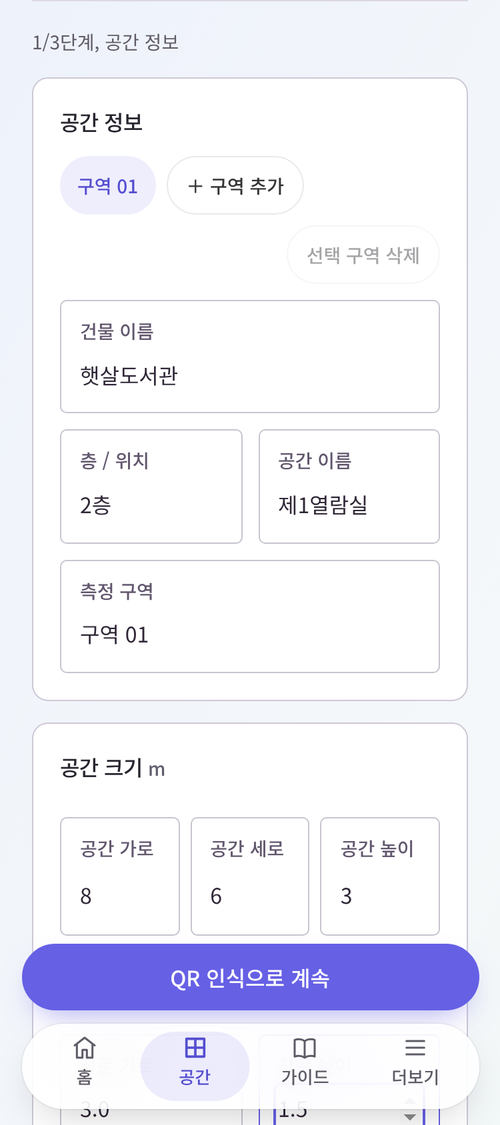
\includegraphics[width=0.46\columnwidth]{fig_register_a.png}\hfill
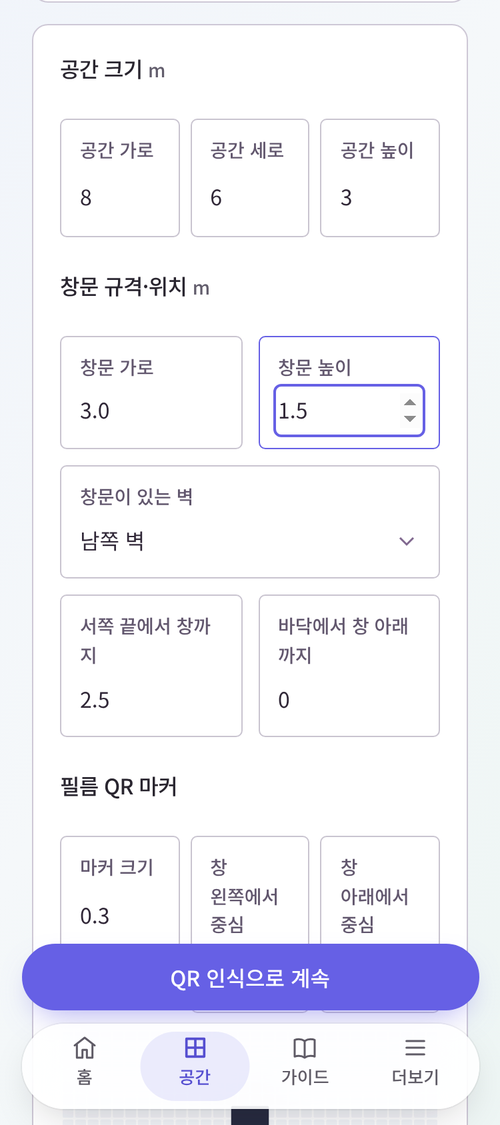
\includegraphics[width=0.46\columnwidth]{fig_register_b.png}
\caption{Space registration screen (Korean-language interface of the prototype): space information (left), room size, window and marker (right).}
\label{fig:register}
\end{figure}

\subsubhead{Scene Storage and Versioning}
\noindent\hspace*{\parindent}A Scene (version 0.2.0) is the shared description of a space. It holds a site (latitude, longitude, time zone), a room, windows, furniture boxes, protected areas, markers and observation records. The server validates every Scene before it is stored and keeps a revision number, so that two users cannot overwrite each other's changes.

\TR
\begin{itemize}
\item Objects: room (floor polygon, height, floor level); window (corners, axes, film grid); furniture (box, yaw, type); protected area (rectangle, normal, grade); marker (ID, size, transform, cell block); observation (source, time, uncertainty)
\item Optional fields (film grid, marker position, furniture type, floor level) have defaults, so that older Scenes remain valid
\item Validation: finite numbers, a planar floor polygon, rectangular windows and protected areas, windows on walls, furniture inside the room, normals, unique IDs, references between objects; an invalid Scene returns 422 with the location and an explanation, and the stored data stay unchanged
\item Revision: the revision increases by one on every update; \texttt{PUT /api/scenes/\allowbreak\{id\}} succeeds only if the revision in the database is still the one that the client has read, and otherwise returns 409
\item Routes: \texttt{POST /api/scenes/\allowbreak validate}, \texttt{GET /api/\allowbreak scene-schema}, \texttt{POST} and \texttt{GET /api/scenes}, \texttt{GET} and \texttt{PUT /api/scenes/\allowbreak\{id\}}
\item Data of the screens (building, floor, zone) are stored in a separate table in the same transaction as the Scene, so that the Scene contract is not changed
\item Both applications read and write the same Scene through these routes, so a space saved on one device appears on the other after the next read (NFR3.1)
\end{itemize}

\subsubhead{Floor Plan Check and Protected Area Editing}
\noindent\hspace*{\parindent}After the measurement, the user checks the floor plan, corrects the furniture and defines the protected areas. The protected areas can be defined and edited in the mobile application as well as on the web.

\TR
\begin{itemize}
\item Furniture: type, width, depth, height and position can be changed; furniture can be dragged on the 2D plan, added and deleted; each type has its own plan symbol, and the window is drawn at its real position
\item Protected area: created from a face of a piece of furniture or by drawing a rectangle; start and end height; grade A to D; moved and resized by dragging or by numbers
\item If the server refuses a revision (409), the screen offers the newest content
\item The edit screen shows whether there are unsaved changes and asks for a confirmation before the user leaves it; a screen without changes closes without a question
\end{itemize}

\begin{figure}[!t]
\centering
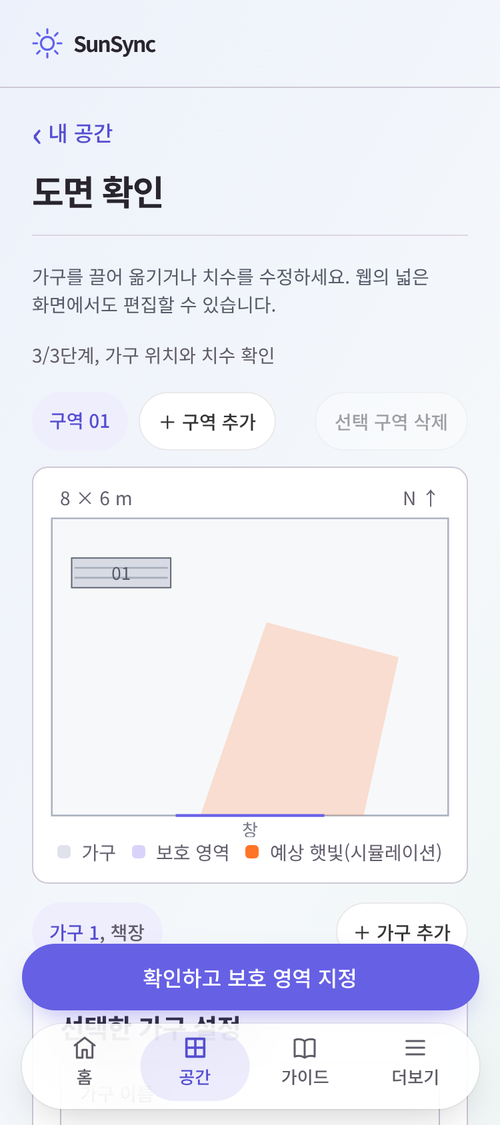
\includegraphics[width=0.46\columnwidth]{fig_plan_a.png}\hfill
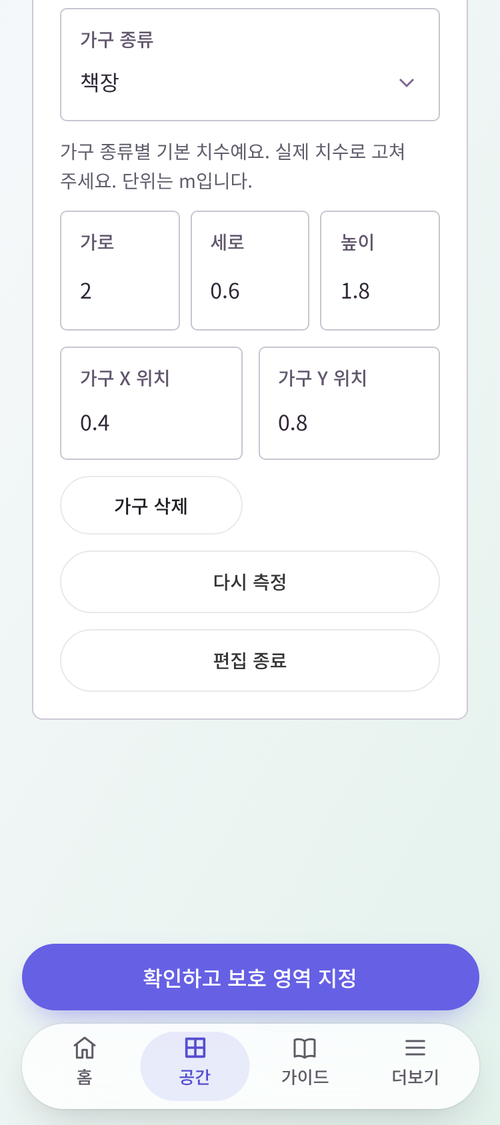
\includegraphics[width=0.46\columnwidth]{fig_plan_b.png}
\caption{Floor plan check: the 2D plan with the window (left) and the editing of a piece of furniture (right).}
\label{fig:plan}
\end{figure}

\begin{figure}[!t]
\centering
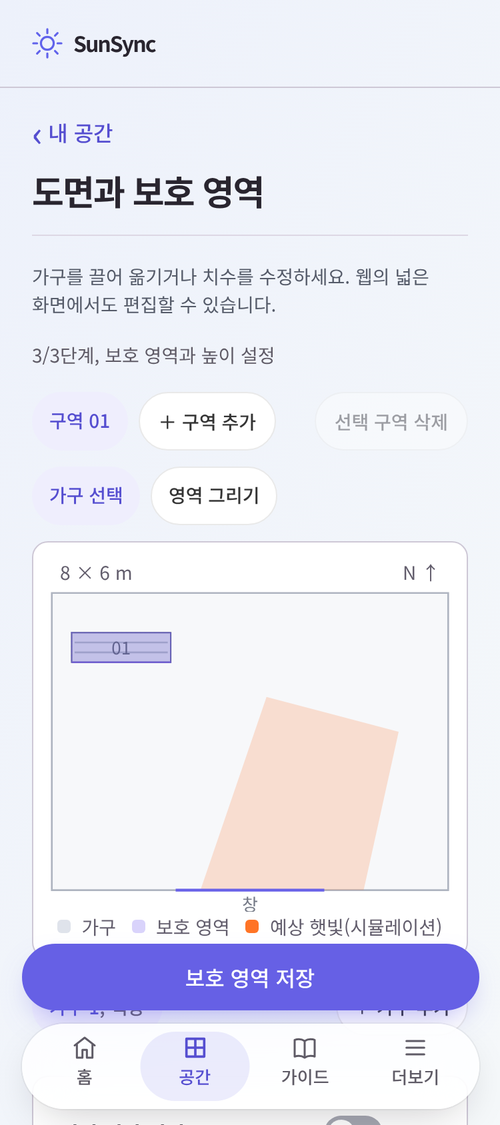
\includegraphics[width=0.46\columnwidth]{fig_protect_a.png}\hfill
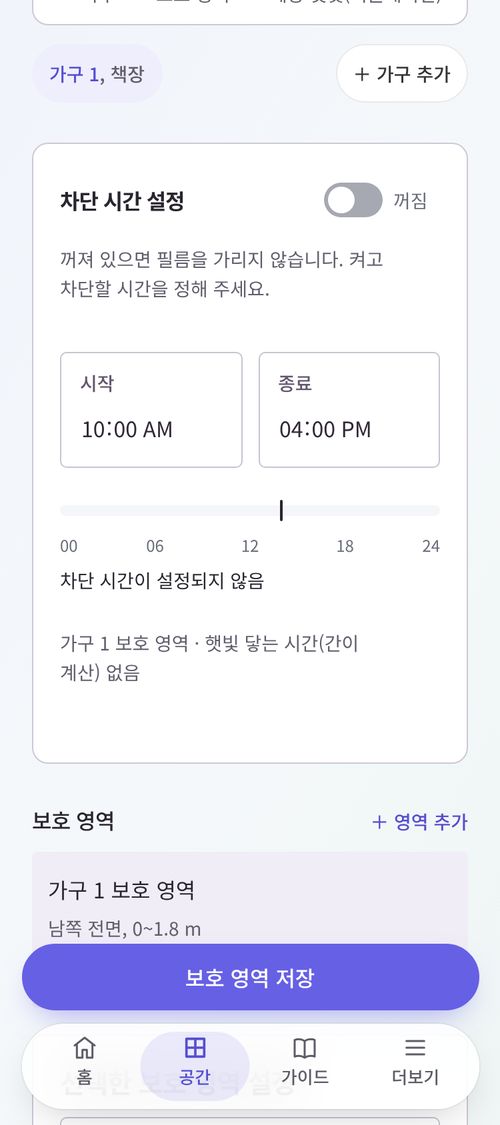
\includegraphics[width=0.46\columnwidth]{fig_protect_b.png}
\caption{Protected areas and shading hours: selecting a furniture face or drawing an area (left), shading hours and the list of areas with grades (right).}
\label{fig:protect}
\end{figure}

\begin{figure*}[!t]
\centering

\includegraphics[width=0.48\textwidth]{fig_web_edit.png}\hfill
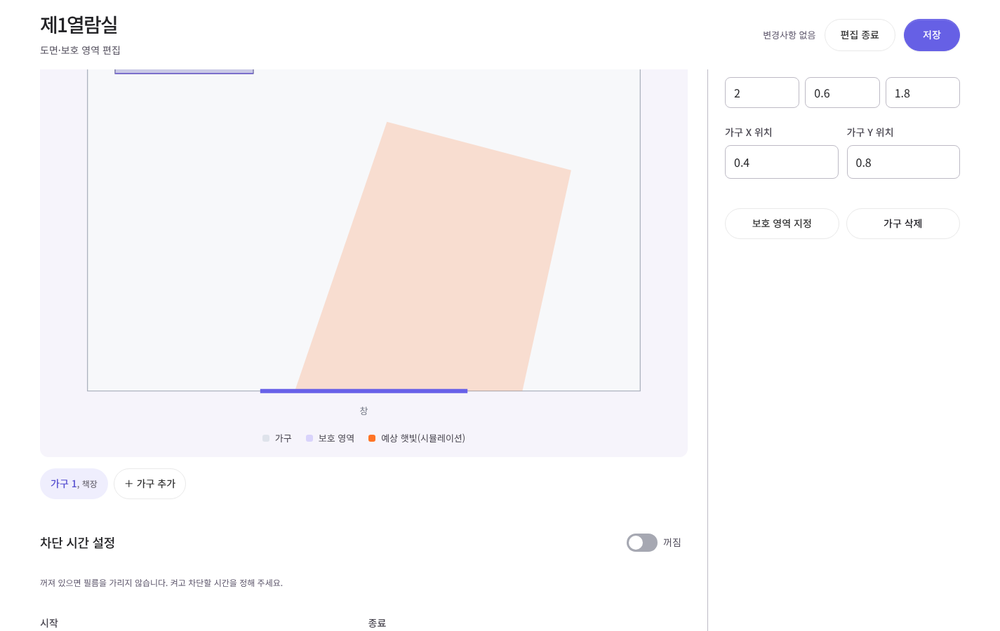
\includegraphics[width=0.48\textwidth]{fig_web_edit_b.png}
\caption{Web application: editing of the floor plan, furniture and shading hours (the protected areas are drawn on the same plan).}
\label{fig:webedit}
\end{figure*}

\subsubhead{3D View (planned)}
\noindent\hspace*{\parindent}The web application shows the measured space in 3D, so that the user can check the room, the window and the furniture from any side. The 3D view is planned and is not implemented yet.

\TR
\begin{itemize}
\item The view is drawn with Three.js \cite{threejs} from the same Scene as the 2D plan, in the ENU frame with $z$ up, so that no conversion between the plan and the 3D view is needed
\item Room: floor polygon extruded to the room height; window: rectangle on its wall with the film grid; furniture: a box of the size, yaw and type from the Scene, drawn with a default shape for each type (bookshelf, desk, chair, other)
\item Furniture can be dragged on the floor; the new position is checked against the room and saved with \texttt{PUT /api/scenes/\allowbreak\{id\}} and the revision that the client has read (409 on a conflict)
\item The sunlight and the film cells of the selected time (Section IV-F) are planned as an overlay on the same view
\end{itemize}

\subsubhead{Protection Grades}
\noindent\hspace*{\parindent}The grade of a protected area tells the system how strictly direct sunlight must be blocked.

\TR
\begin{itemize}
\item Grade A: every geometric direct-sun path to the surface must pass through an opaque cell, even if the predicted intensity is low or unknown
\item Grades B and C: the direct irradiance on the surface is limited to a low and a higher configurable value, with $0<B<C$ (30 and 70 W/m$^2$ in the demonstration); the metric is the direct irradiance in W/m$^2$, and the maximum over the sample points of the area is used
\item Grade D: priority to daylight, no shading request
\end{itemize}

\gapsubsection
\subsection{Sunlight Prediction Features}
\subsubhead{Time Grid and Solar Position}
\noindent\hspace*{\parindent}FR-01 predicts the exposure of protected areas on a grid of future time steps for a stored Scene.

\TR
\begin{itemize}
\item Request: a stored Scene, a start time with a time zone offset, a duration (default 120 min, 1 to 1440) and a time step (default 300 s, 1 to 3600); optional region IDs and expected Scene revision
\item Limits: at most 1,441 time steps and 10,000 sample points; a request is rejected if the number of time steps $\times$ sample points $\times$ (windows + furniture boxes + room edges + 2) exceeds $5\times10^{6}$
\item Sun position: pvlib with the NREL algorithm, altitude 0 and a pressure of 101,325 Pa; the geometric elevation $h$ and the azimuth $a$ (clockwise from north) give the unit vector toward the sun, $\mathbf{s}=(\cos h\sin a,\ \cos h\cos a,\ \sin h)$
\item If $h\le 0$, the sun is below the horizon and no tile is exposed
\end{itemize}

\subsubhead{Direct-Sun Path Tracing}
\noindent\hspace*{\parindent}A ray is traced from the centre of every tile of a protected area toward the sun. The point is exposed if the ray leaves the room through a window.

\TR
\begin{itemize}
\item Tiles: each rectangular protected area is divided along its two edges into tiles of 5 cm $\times$ 5 cm; a last tile that is shorter than 5 cm is kept with its remaining width; tiles are numbered row by row
\item The ray must cross a window aperture before the nearest wall, floor, ceiling or furniture box; boxes are intersected with the slab method \cite{kay} in their own rotated frame
\item Reasons for not exposed: \texttt{sun\_below\_horizon}, \texttt{back\_facing}, \texttt{no\_window}, \texttt{window\_missed}, \texttt{boundary\_ambiguous}, \texttt{room\_blocked}, \texttt{occluder\_blocked}; a crossing on the edge of an aperture is ambiguous and counts as not exposed
\item Reflection, scattering, window transmittance, window frames, walls with thickness and objects outside the building are not modeled
\end{itemize}

\noindent\hspace*{\parindent}Algorithm~\ref{alg:fr01} summarizes the procedure.

\begin{algorithm}[!t]
\caption{FR-01 Prediction}
\label{alg:fr01}
\small
\begin{algorithmic}[1]
\Require Scene, start $t_0$, duration, step $\Delta$
\State $T \gets$ UTC grid from $t_0$ with step $\Delta$
\For{each $t_k \in T$}
  \State $(h_k,a_k) \gets$ pvlib sun position; $\mathbf{s}_k$
  \State $d_k \gets$ SelectDNI$(t_k)$
\EndFor
\For{each region $R$, each tile centre $\mathbf{p}$ of $R$}
  \For{each $t_k \in T$}
    \If{$h_k \le 0$}
      \State not exposed: sun\_below\_horizon
    \ElsIf{$\mathbf{n}_R\cdot\mathbf{s}_k \le \epsilon$}
      \State not exposed: back\_facing
    \Else
      \State $w \gets$ window hit by ray $\mathbf{p}+\tau\mathbf{s}_k$
      \State $b \gets$ nearest wall, floor or ceiling hit
      \State $o \gets$ nearest furniture hit
      \If{$w$ exists, $w$ is before $b$ and $o$}
        \State exposed; keep $w$, hit point, $E$
      \Else
        \State not exposed with the matching reason
      \EndIf
    \EndIf
  \EndFor
\EndFor
\State summarize each region (first exposure, intervals)
\end{algorithmic}
\end{algorithm}

\subsubhead{Direct Sunlight Intensity}
\noindent\hspace*{\parindent}FR-01.4 selects the strength of the sunlight for every time step and converts it to the direct irradiance on each tile.

\TR
\begin{itemize}
\item Selection for each time step, independently of the other steps: (1) a valid weather record in the Scene, (2) the stored Open-Meteo forecast whose hour contains the step, (3) the pvlib clear-sky DNI, otherwise \texttt{unknown}
\item A worker requests \texttt{direct\_normal\_irradiance} and \texttt{cloud\_cover} for each stored location and saves the hourly values with the fetch time and the forecast grid point; the value of an hour applies to the hour that ends at its time stamp
\item A prediction request only reads the stored records and never calls the service, so a failure of the service does not stop a prediction
\item Irradiance on an exposed tile: $E = d\cdot\max(0,\mathbf{n}\cdot\mathbf{s})$ in W/m$^2$, with the selected DNI $d$ and the receiving normal $\mathbf{n}$; a tile that is not exposed has $E=0$; an exposed tile with unknown DNI has $E=\texttt{null}$
\end{itemize}

\subsubhead{Prediction Interface}
\noindent\hspace*{\parindent}The prediction is requested for a stored Scene and is not stored.

\TR
\begin{itemize}
\item Route: \texttt{POST /api/scenes/\allowbreak\{scene\_id\}/\allowbreak sunpath-predictions}
\item Response: for every region and time step, the status, reason, window, crossing point and $E$ of each sample point; the number of exposed tiles; the first predicted exposure time; the merged exposure intervals; the source of the DNI of each step; the first exposure is a time step of the grid, and nothing is interpolated between two steps
\item Errors: 404 for a missing Scene, 409 for another revision, 422 for an invalid request or an exceeded limit
\item Verification: a synthetic Scene near Seoul City Hall is checked against hand-calculated values (NFR1.1)
\end{itemize}

\subsubhead{Performance and Reproducibility}
\noindent\hspace*{\parindent}The prediction must be fast enough for an interactive screen (NFR2.1) and must give the same result for the same input (NFR3.1).

\TR
\begin{itemize}
\item Bounded work: the limits of the request (at most 1,441 time steps, 10,000 sample points and $5\times10^{6}$ for the product of time steps, sample points and geometry objects) are checked before the calculation starts; the default plan of two hours with a step of 300 s has 25 time steps
\item No external call in a request: the forecast is read from the database, so the run time does not depend on the network
\item Check of NFR2.1: the run time of a two-hour plan for one zone is measured on the development computers and compared with 5 s
\item Reproducibility: the time grid is built in UTC, the solar position uses fixed parameters of the algorithm, the tiles are numbered in a fixed order, and among several forecast snapshots for one hour the most recent fetch and then a fixed order of the snapshot ID is used, so the same Scene, request and stored forecast give the same result
\end{itemize}

\gapsubsection
\subsection{Shading Decision Features}
\subsubhead{Cell Mapping}
\noindent\hspace*{\parindent}FR-02.1 converts the window crossing points of FR-01 to film cells.

\TR
\begin{itemize}
\item Input: only the tiles that are exposed with reason \texttt{clear\_path} and have a window and a crossing point
\item The crossing point $\mathbf{q}$ becomes window coordinates $u=(\mathbf{q}-\mathbf{o})\cdot\mathbf{u}$ and $v=(\mathbf{q}-\mathbf{o})\cdot\mathbf{v}$ with the origin at the top-left corner
\item A square of 5 cm $\times$ 5 cm around $(u,v)$ is clipped to the window, and every cell that it overlaps with a positive area is selected; a point near a boundary selects two or more cells; a point outside the window selects none and causes no error
\item The cell size is taken from the window, not fixed to 10 cm
\end{itemize}

\subsubhead{Grade-Based Decision}
\noindent\hspace*{\parindent}FR-02.2 decides, for every cell, area and time step, whether the cell is needed and in which state.

\TR
\begin{itemize}
\item Grade A: every cell that a path reaches is needed, whatever the intensity; if the film cannot block fully (its minimum transmittance is above zero), the state is \texttt{infeasible}
\item Grades B and C: the largest $E$ of the tiles of the area that map to the cell is compared with the limit of the grade; at or below the limit nothing is needed; above it, the state is \texttt{opaque} if the darkest film state brings the intensity to the limit or below, and \texttt{infeasible} otherwise
\item If $E$ is unknown, the state is \texttt{unknown} and not zero, unless a known tile is already above the limit
\item Grade D: no need
\item Several areas in one cell: the most severe state applies in the order \texttt{infeasible}, \texttt{opaque}, \texttt{unknown}, because a darker cell never harms another area; all active areas are listed as reasons, strictest grade first
\item Margin: a need at step $t_k$ covers $[t_k-\Delta,\ t_k+\Delta)$, cut at the period of the plan (see Advance Shading)
\end{itemize}

\noindent\hspace*{\parindent}Algorithm~\ref{alg:fr02} summarizes the procedure.

\begin{algorithm}[!t]
\caption{FR-02 Decision}
\label{alg:fr02}
\small
\begin{algorithmic}[1]
\Require FR-01 result, window grids, grades, limits
\For{each step $t_k$, region $R$}
  \For{each exposed clear\_path tile $x$ of $R$}
    \State add Cells$(x)$ to $C_{R,k}$
  \EndFor
  \For{each cell $c \in C_{R,k}$}
    \State $n \gets$ Need$(R, c, k)$ by the grade rules
    \If{$n$ exists}
      \State add $(n, R, \text{grade})$ to needs of $(c,k)$
    \EndIf
  \EndFor
\EndFor
\For{each cell $c$ and step $t_k$ with needs}
  \State state $\gets$ most severe state of its needs
  \State reasons $\gets$ its areas, strictest grade first
  \State cover $[t_k-\Delta,\ t_k+\Delta)$ cut to the period
\EndFor
\State merge equal neighbours; split where state or reasons change
\State \Return ShadingPlan
\end{algorithmic}
\end{algorithm}

\subsubhead{Advance Shading}
\noindent\hspace*{\parindent}FR-02.3 requires that a cell is switched before the sunlight arrives, allowing for the switching time of the film, the processing delay and a safety margin.

\TR
\begin{itemize}
\item Current realization: a need at step $t_k$ is planned from $t_k-\Delta$, one time step before the sampled arrival, because the sun may arrive anywhere between two steps; the default step is 300 s
\item The switching time of PDLC film is 10 to 150 ms \cite{gauzypdlc}, so the one-step margin covers it with a large reserve
\item Planned parameters of the plan request: the switching time of the film $\tau_\mathrm{sw}$, the processing delay $\tau_\mathrm{proc}$ and a safety margin $\tau_\mathrm{margin}$; the lead $\lambda=\tau_\mathrm{sw}+\tau_\mathrm{proc}+\tau_\mathrm{margin}$ replaces the one-step margin only if it is longer than $\Delta$
\item An exposure that starts and ends between two steps is not seen; a smaller time step reduces this risk
\end{itemize}

\subsubhead{Shading Plan and Interface}
\noindent\hspace*{\parindent}FR-02.4 returns the decision as one shading plan per Scene, which FR-05 and the screens read.

\TR
\begin{itemize}
\item Structure: Scene and revision, period, windows; each window lists its cells; each cell lists segments with start, end, state and reasons (area ID and grade); version 0.1.0
\item States: \texttt{opaque}, \texttt{transparent}, \texttt{infeasible}, \texttt{unknown}; a window or cell that is not listed is transparent for the whole plan; a segment covers its start but not its end
\item The model rejects unknown fields, overlapping or unordered segments, cells outside the grid, duplicates, segments outside the period, and a needed state without a reason
\item Route: \texttt{POST /api/scenes/\allowbreak\{scene\_id\}/\allowbreak shading-plans} with the fields of the FR-01 request; it runs the FR-01 prediction with the same limits and applies the rules above
\item All protected areas are planned, because a plan for some areas would leave the others unprotected
\item Errors: 404 for a missing Scene, 409 for another revision, 422 for an invalid request or a Scene without protected areas
\end{itemize}

\gapsubsection
\subsection{Film Control Features}
\subsubhead{Virtual Film Device}
\noindent\hspace*{\parindent}FR-05 hides the film behind a device interface, so the simulated film can be replaced by a real controller without changing the decision modules.

\TR
\begin{itemize}
\item Interface: read the opacity of a cell, read the whole grid, and apply a list of cell commands, which returns the previous and the new opacity of each cell
\item The opacity is a number from 0 (transparent) to 1 (opaque); a value in between is dimmed; a PDLC film uses only 0 and 1, and an SPD film can use the whole range
\item The grid size is not fixed to $10\times10$; a cell outside the grid or an opacity outside 0 to 1 is rejected
\item Manual commands: \texttt{POST /api/scenes/\allowbreak\{scene\_id\}/\allowbreak film-commands}; current state: \texttt{GET film-state}
\end{itemize}

\subsubhead{Plan Playback and Application Log}
\noindent\hspace*{\parindent}The plan of FR-02 is applied to the film at the scheduled times, and every change is recorded.

\TR
\begin{itemize}
\item Mapping of the plan states: \texttt{transparent} gives opacity 0; \texttt{opaque} gives 1; \texttt{infeasible} gives 1 with status \texttt{target\_unmet}; \texttt{unknown} gives 1 with status \texttt{unknown\_intensity}
\item A segment that enters \texttt{infeasible} writes its log entry even if the cell was already opaque
\item Each log entry holds the time, window, cell, previous and new opacity and state, status, note, the reasons (areas and grades) and the plan ID; the log is append-only
\item Route: \texttt{POST film-schedule-apply} computes the plan for the given request and applies it; applying the same plan ID again replaces its own log entries and does not duplicate them; a plan with another ID keeps the earlier logs and becomes the active plan
\item Simulation clock: \texttt{GET film-state?at=} returns the state at any time, computed from the active plan, or by replaying the log if no plan is active; a time without a time zone offset gives 422, so that a demonstration can show a whole day in a few seconds
\item Log query: \texttt{GET film-logs} with filters for status and time; all times are stored in UTC, so that string order equals time order
\end{itemize}

\noindent\hspace*{\parindent}Algorithm~\ref{alg:fr05} summarizes the playback.

\begin{algorithm}[!t]
\caption{FR-05 Applying a Plan}
\label{alg:fr05}
\small
\begin{algorithmic}[1]
\Require Scene id, ShadingPlan with plan id
\State delete the log entries of the same plan id
\For{each window, cell and segment in time order}
  \State $(o,\text{status}) \gets$ mapping of the plan state
  \State apply opacity $o$ at the segment start
  \State append log: time, cell, previous and new opacity,
  \Statex \hspace{\algorithmicindent} status, reasons, plan id
\EndFor
\State store the plan as the active plan of the film
\end{algorithmic}
\end{algorithm}

\subsubhead{Marker Display}
\noindent\hspace*{\parindent}FR-05.2 displays the marker board of FR-03 on a block of film cells during a measurement. % NOTE: the film marker mode is planned to change from one 6x6-cell marker to the FR-03 board of four markers

\TR
\begin{itemize}
\item Route: \texttt{POST film-marker-mode} with an \texttt{enabled} flag, a marker code and a start cell (default row 2, column 2)
\item When enabled, the opacities of all cells are saved, and the marker board of FR-03 (four ArUco markers of the $4\times4$ dictionary in a $2\times2$ arrangement, each with a border) is drawn on the block of cells that it occupies; the block and the marker codes are parameters of the command
\item When disabled, the saved opacities are restored; changes made outside the marker area in the meantime are kept
\end{itemize}

\gapsubsection
\subsection{Spatial Measurement Features}
\subsubhead{Measurement Request}
\noindent\hspace*{\parindent}A measurement is a job that belongs to the account of the user. It can be requested on the web or in the mobile application and is carried out with the phone, so that the user does not have to type a connection code or an address.

\TR
\begin{itemize}
\item Flow: the user requests a measurement for a space; the server stores the job; the mobile application lists the waiting job with the space; the user starts the capture; the result is saved to the Scene; the web application shows the measurement as completed and opens the floor plan
\item Routes under \texttt{/api/ui/measurements}: create and list jobs; \texttt{/\{token\}} for the state and the space; \texttt{/\{token\}/connect} to start the capture; \texttt{/\{token\}/complete} to check the saved revision and finish the job
\item A second active request for the same space returns the existing job; the list of spaces refreshes the jobs every 3 seconds
\item A link or a QR code can open a job directly on the phone, and it is hidden when the address of the server is \texttt{localhost}; the camera and the position of the device need HTTPS
\item The real checking of an account and the separation of the jobs by user have to be provided by the account layer of the server (Section IV-A)
\end{itemize}

\subsubhead{Guided Capture}
\noindent\hspace*{\parindent}The application guides the user through the photos; the measurement module is a platform-independent Python module with its own HTTP interface that does not store images. The application passes the camera parameters of every frame, because the pose cannot be computed without them.

\TR
\begin{itemize}
\item Plan: the module returns the measuring points $P_1,\dots,P_n$, their order and the number of repetitions for the type, model and top shape of the furniture; for a rectangular top the points are its four corners
\item Capture: at each point the user holds the phone with the lens at the point and photographs the marker; the application fixes the point ID and the capture time when the shutter is pressed, and rejects a late answer for another point
\item Detection: the module returns the corner pixels of the marker and whether the pose is valid; a photo in which the marker is not fully visible or the same marker ID appears twice is rejected, and the user retakes it
\item Camera parameters: image size, focal lengths, principal point, distortion and the pixel space (raw or rectified); images are not rotated by EXIF
\item Result: after the last photo the application sends the measurement data to the server and shows the progress of the floor plan generation, which the user can cancel
\end{itemize}

\begin{figure}[!t]
\centering
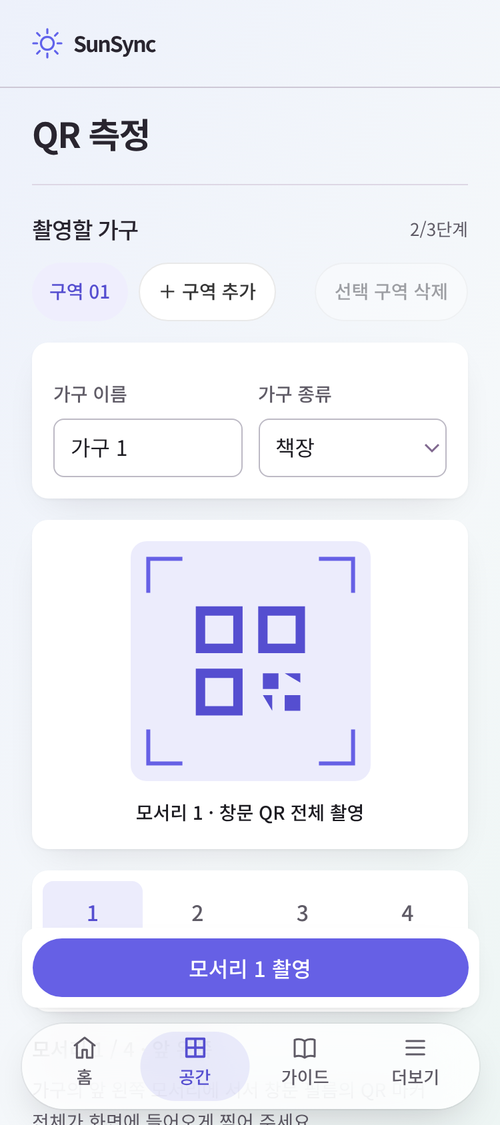
\includegraphics[width=0.46\columnwidth]{fig_capture_a.png}\hfill
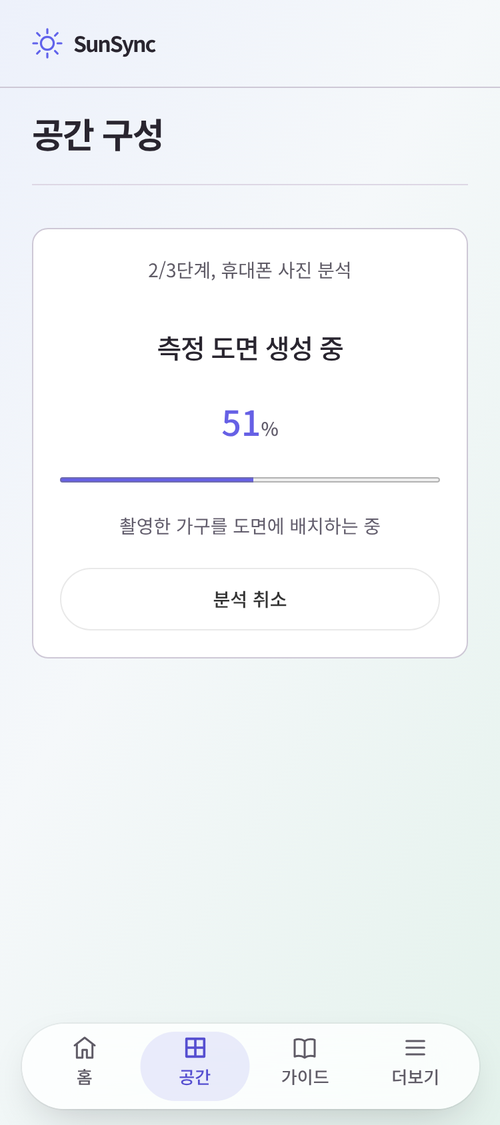
\includegraphics[width=0.46\columnwidth]{fig_capture_b.png}
\caption{Corner capture (left) and the progress of the floor plan generation (right).}
\label{fig:capture}
\end{figure}

\subsubhead{Pose and Furniture Shape}
\noindent\hspace*{\parindent}The module computes the coordinates of the measuring points and the shape of the furniture.

\TR
\begin{itemize}
\item Marker: ArUco markers of the $4\times4$ dictionary with known size and spacing; the origin is the top-left corner of the top-left marker
\item Pose: solvePnP from all marker corners; the server computes the pose again from the submitted corners and does not trust 3D coordinates of the client
\item Point: the optical centre of the camera is the coordinate of the point, corrected by the vector from the lens to the contact point if it is known
\item Quality: ambiguity of the pose, reprojection error, deviation between repeated photos of a point, residual of the fitted plane and shape, horizontality of the top; a point that fails is photographed again
\item Shapes: rectangle (4 points), circle (4), ellipse (6), simple polygon (3 to 16)
\item Height from the floor reference: the top is the highest part, an extra photo of the highest point, or a manual measurement; floating furniture also needs its installation height
\item Conversion to ENU with the $4\times4$ transform of the board; the north direction, the room origin and the floor reference must be confirmed
\end{itemize}

\noindent\hspace*{\parindent}Algorithm~\ref{alg:fr03} summarizes the procedure.

\begin{algorithm}[!t]
\caption{FR-03 Furniture Measurement}
\label{alg:fr03}
\small
\begin{algorithmic}[1]
\Require points $P_1,\dots,P_n$, marker, camera data
\For{each point $P_i$ and repetition}
  \State corners $\gets$ DetectMarker(photo)
  \If{marker not fully visible}
    \State \Return retake request for $P_i$
  \EndIf
  \State $(R,\mathbf{t}) \gets$ solvePnP(corners, size, camera)
  \State $\mathbf{p}_i \gets -R^{\top}\mathbf{t}$ (camera centre)
\EndFor
\If{pose, spread or residual checks fail}
  \State \Return retake request for the failing points
\EndIf
\State shape $\gets$ Fit$(\{\mathbf{p}_i\})$; height by chosen mode
\State \Return size and placement in ENU
\end{algorithmic}
\end{algorithm}

\subsubhead{Registration in the Scene}
\noindent\hspace*{\parindent}The result is added to the Scene through the server.

\TR
\begin{itemize}
\item The module exports a fragment with its own format version; it is sent to \texttt{POST /api/scenes/\allowbreak\{scene\_id\}/\allowbreak registrations} together with the revision that the client has read
\item The server checks the transforms, the consistency of size, centre, yaw and height, the horizontal top and the position inside the room; it adds the furniture box with an observation record (capture time, height mode, model ID) and increases the revision once; another revision gives 409 and an inconsistent input gives 422, and the stored Scene stays unchanged
\item The registration is limited to cuboids with a rectangular top; circles, ellipses and polygons can be measured but are rejected on export; the furniture box is the bounding box of the model, so the space between table legs is filled
\item Limit: the module has been verified with synthetic photos from known camera and board positions, which does not verify the accuracy with real photos; an earlier experiment had a horizontal error of about 10.6\% % TODO: confirm with Daeun Lee; also how the board relates to the marker shown on the film
\end{itemize}

\gapsubsection
\subsection{Space Status Features}
\subsubhead{Space Status Display}
\noindent\hspace*{\parindent}The space status screen shows the result of the prediction and the shading decision for a selected day.

\begin{figure}[!t]
\centering
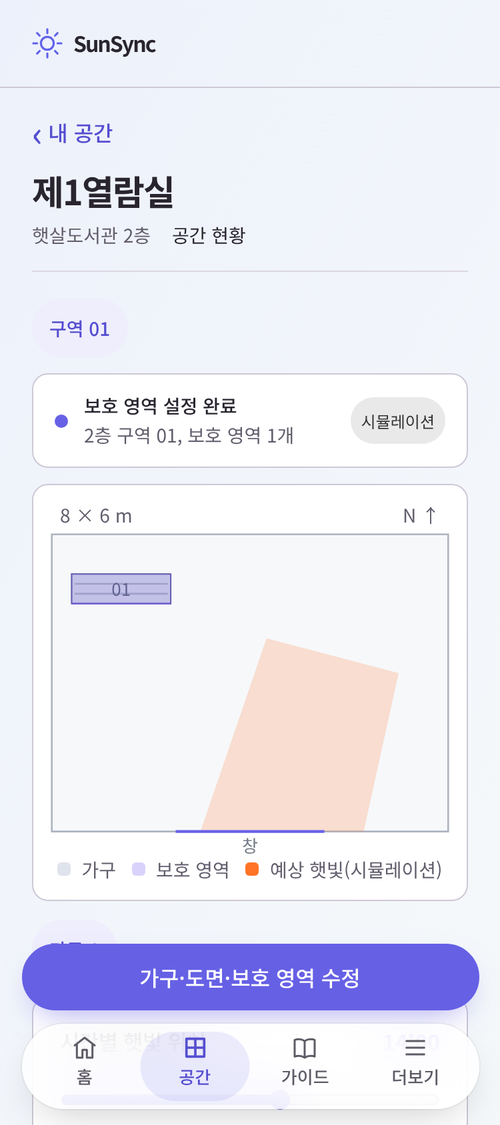
\includegraphics[width=0.46\columnwidth]{fig_status_a.png}\hfill
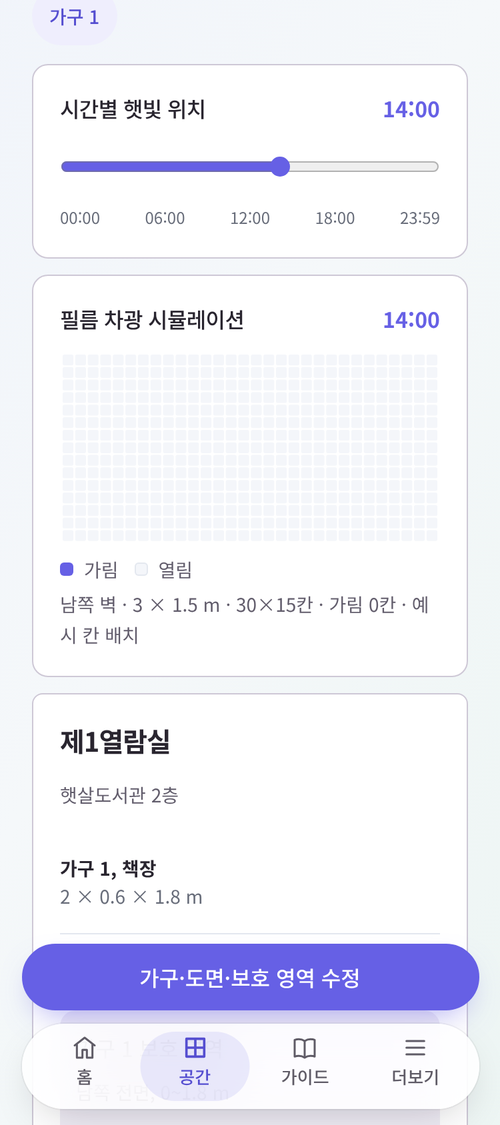
\includegraphics[width=0.46\columnwidth]{fig_status_b.png}
\caption{Space status: the plan with the predicted sunlight (left), the time slider and the film grid of the window (right). The sunlight and the film cells in this prototype screen are example values.}
\label{fig:status}
\end{figure}

\begin{figure*}[!t]
\centering
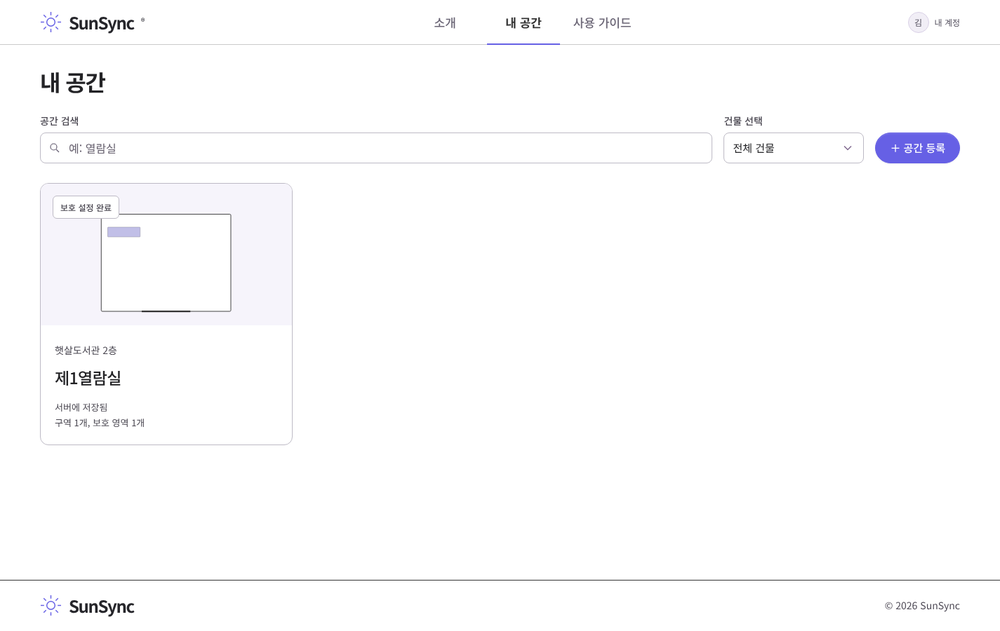
\includegraphics[width=0.48\textwidth]{fig_web_spaces.png}\hfill
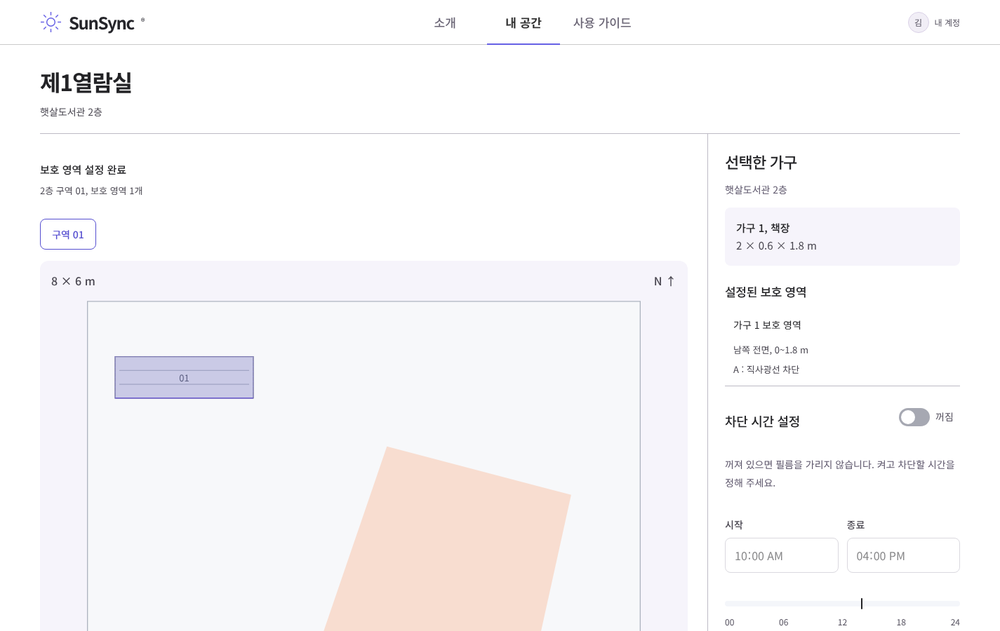
\includegraphics[width=0.48\textwidth]{fig_web_status.png}
\caption{Web application: the list of spaces (left) and the space status with the plan and the shading hours (right).}
\label{fig:webstatus}
\end{figure*}

\TR
\begin{itemize}
\item The prediction is requested for a saved space whose north direction is confirmed, pinned to the revision of the Scene, for a full day at 30-minute steps
\item The screen shows the first sampled exposure and the peak sampled irradiance of each region, and whether the intensity comes from a forecast, the clear-sky value or is missing; 0 is shown as a physical value and \texttt{null} as unknown
\item A time slider selects the time; the window is drawn as a grid of film cells and the cells that are opaque at that time are highlighted
\item Shading hours: the user turns shading on or off and sets the start and end time in steps of 10 minutes (start before end); the film is shaded only within these hours; grade D is never shaded
\item Blocking times: for each protected area the screen shows the first time at which light toward the area is expected to be blocked, taken from the shading plan, or ``no blocking expected today''; a recalculation button requests the plan again for the saved revision, shows a loading state while it runs and an error message if it fails; changes of the space or of an area appear at the next request
\end{itemize}

\subsubhead{User Guide and Account}
\noindent\hspace*{\parindent}A step-by-step guide explains the registration, the measurement, the protected areas and the shading hours; the web and the mobile application share its content. The account screen shows the account and the registered spaces, zones and protected areas.

\TR
\begin{itemize}
\item The guide lists the steps, explains one step per screen with previous and next buttons, and does not start a measurement or an edit; closing the help during a task returns to the task
\item The account screen offers sign out with a confirmation; the screens and the browser history keep the entered values when the user goes back
\end{itemize}





\begin{thebibliography}{00}
\bibitem{nedcc} Northeast Document Conservation Center, ``2.4 Protection from light damage,'' Preservation Leaflets. [Online]. Available: \url{https://nedcc.org/free-resources/preservation-leaflets/2.-the-environment/2.4-protection-from-light-damage}
\bibitem{cci} Canadian Conservation Institute, ``Agent of deterioration: Light, ultraviolet and infrared,'' Government of Canada. [Online]. Available: \url{https://www.canada.ca/en/conservation-institute/services/agents-deterioration/light.html}
\bibitem{cam} University of Cambridge, ``Libraries and light,'' Research News. [Online]. Available: \url{https://www.cam.ac.uk/research/news/libraries-and-light}
\bibitem{solargard} Solar Gard, ``Brown University: Panorama window film success story,'' case study. [Online]. Available: \url{https://www.solargard.com/wp-content/uploads/2016/02/brown-university-panorama-success-story-pdf0163panl.pdf}
\bibitem{view} View, Inc., ``Introducing View Intelligence 2.0.'' [Online]. Available: \url{https://www.view.com/blog/introducing-view-intelligence-2-0}
\bibitem{lgchem} LG Corp., ``LG Chem enters the automotive switchable film market,'' press release, 2024. [Online]. Available: \url{https://www.lg.co.kr/media/release/27620}
\bibitem{gauzyces} Gauzy, ``Gauzy's 2022 CES experience,'' 2022. [Online]. Available: \url{https://www.gauzy.com/internal_news/2022-ces-experience/}
\bibitem{patent} L.-Y. Yeh, A. Fessemaz, N. Hecker, and F. Jacques, ``Segmented multilayer film with electrically controllable optical properties,'' U.S. Patent 12\,181\,741 B2, Dec. 31, 2024. [Online]. Available: \url{https://patents.google.com/patent/US12181741}
\bibitem{pvlib} W. F. Holmgren, C. W. Hansen, and M. A. Mikofski, ``pvlib python: A python package for modeling solar energy systems,'' J. Open Source Softw., vol. 3, no. 29, p. 884, 2018.
\bibitem{reda} I. Reda and A. Andreas, ``Solar position algorithm for solar radiation applications,'' Solar Energy, vol. 76, no. 5, pp. 577--589, 2004.
\bibitem{gauzypdlc} Gauzy, ``What's the difference between PDLC and SPD smart glass?'' [Online]. Available: \url{https://www.gauzy.com/liquid-crystal-spd-smart-glass-whats-the-difference/}
\bibitem{solarscreen} Solarscreen, ``PDLC vs SPD smart glass differences.'' [Online]. Available: \url{https://solarscreen.eu/en/blog/pdlc-vs-spd-smart-glass-differences}
\bibitem{sageglass} Saint-Gobain, ``SageGlass LightZone'' and ``SageGlass Harmony'' product pages. [Online]. Available: \url{https://www.saint-gobain.com.cn/en/glass/product/sageglass-lightzone}
\bibitem{mecho} ``SolarTrac from MechoShade Systems,'' Architect Magazine. [Online]. Available: \url{https://www.architectmagazine.com/technology/solartrac-from-mechoshade-systems_o/}
\bibitem{thinq} LG Electronics, ``LG opens new chapter in connected home living with `ThinQ ON' AI home hub at IFA 2024,'' press release, Aug. 2024. [Online]. Available: \url{https://www.aap.com.au/aapreleases/cision20240828ae93244/}
\bibitem{radiance} G. J. Ward, ``The RADIANCE lighting simulation and rendering system,'' in Proc. SIGGRAPH, 1994, pp. 459--472.
\bibitem{python} ``Python documentation.'' [Online]. Available: \url{https://docs.python.org/3/}
\bibitem{typescript} ``TypeScript documentation.'' [Online]. Available: \url{https://www.typescriptlang.org/docs/}
\bibitem{github} ``GitHub documentation.'' [Online]. Available: \url{https://docs.github.com}
\bibitem{githubactions} ``GitHub Actions documentation.'' [Online]. Available: \url{https://docs.github.com/actions}
\bibitem{pytest} ``pytest documentation.'' [Online]. Available: \url{https://docs.pytest.org/en/stable/}
\bibitem{ruff} ``Ruff documentation.'' [Online]. Available: \url{https://docs.astral.sh/ruff/}
\bibitem{mypy} ``mypy documentation.'' [Online]. Available: \url{https://mypy.readthedocs.io/en/stable/}
\bibitem{oxlint} ``Oxlint documentation.'' [Online]. Available: \url{https://oxc.rs/docs/guide/usage/linter.html}
\bibitem{overleaf} ``Overleaf documentation.'' [Online]. Available: \url{https://www.overleaf.com/learn}
\bibitem{gdocs} ``Google Docs.'' [Online]. Available: \url{https://workspace.google.com/products/docs/}
\bibitem{fastapi} ``FastAPI documentation.'' [Online]. Available: \url{https://fastapi.tiangolo.com}
\bibitem{react} ``React documentation.'' [Online]. Available: \url{https://react.dev}
\bibitem{vite} ``Vite documentation.'' [Online]. Available: \url{https://vite.dev}
\bibitem{openmeteo} ``Open-Meteo weather forecast API documentation.'' [Online]. Available: \url{https://open-meteo.com/en/docs}
\bibitem{opencv} ``Camera calibration and 3D reconstruction,'' OpenCV documentation. [Online]. Available: \url{https://docs.opencv.org/4.x/d9/d0c/group__calib3d.html}
\bibitem{garrido} S. Garrido-Jurado, R. Mu\~noz-Salinas, F. J. Madrid-Cuevas, and M. J. Mar\'in-Jim\'enez, ``Automatic generation and detection of highly reliable fiducial markers under occlusion,'' Pattern Recognit., vol. 47, no. 6, pp. 2280--2292, 2014.
\bibitem{shapely} ``Shapely user manual.'' [Online]. Available: \url{https://shapely.readthedocs.io}
\bibitem{pydantic} ``Pydantic documentation.'' [Online]. Available: \url{https://docs.pydantic.dev}
\bibitem{sqlmodel} ``SQLModel documentation.'' [Online]. Available: \url{https://sqlmodel.tiangolo.com}
\bibitem{sqlite} ``SQLite documentation.'' [Online]. Available: \url{https://www.sqlite.org/docs.html}
\bibitem{threejs} ``three.js documentation.'' [Online]. Available: \url{https://threejs.org/docs/}
\bibitem{kay} T. L. Kay and J. T. Kajiya, ``Ray tracing complex scenes,'' in Proc. SIGGRAPH, 1986, pp. 269--278.
\end{thebibliography}

\end{document}
